% =====================================================================
% Cross-modality optimal-transport projection of CHD-enhancer chromatin
% onto a 3D MERFISH human fetal heart
%
% Build:    tectonic -X compile chd_enhancer_3d_chromatin_priming.tex
% Bib:      refs.bib (23 entries, semantic citation keys)
% =====================================================================
\documentclass[11pt,a4paper]{article}

% ---- packages --------------------------------------------------------
\usepackage[T1]{fontenc}
\usepackage[utf8]{inputenc}
\usepackage{lmodern}
\usepackage{microtype}
\usepackage[margin=1in]{geometry}
\usepackage{graphicx}
\usepackage{booktabs}
\usepackage{caption}
\usepackage{subcaption}
\usepackage{xcolor}
\usepackage{amsmath,amssymb}
\usepackage{authblk}
\usepackage[round,authoryear]{natbib}
\usepackage{hyperref}
\usepackage{tikz}
\usetikzlibrary{arrows.meta,positioning,shapes.geometric,fit,calc}
\usepackage{titlesec}
\usepackage{enumitem}

\hypersetup{
  colorlinks=true,
  linkcolor=blue!50!black,
  citecolor=teal!60!black,
  urlcolor=blue!50!black
}

\captionsetup{font=small,labelfont=bf,justification=raggedright,singlelinecheck=false}
\titleformat*{\section}{\large\bfseries}
\titleformat*{\subsection}{\normalsize\bfseries}
\setlength{\parskip}{0.4em}
\setlength{\parindent}{0pt}

\renewcommand{\figurename}{Fig.}
\renewcommand{\tablename}{Table}

% ---- title -----------------------------------------------------------
\title{\textbf{Cross-modality optimal-transport projection of\\
CHD-enhancer chromatin onto a 3D MERFISH human fetal heart\\
reveals broad chromatin priming and within-lineage decoupling}}

\author[1]{Anonymous}
\affil[1]{PCW12 Human Fetal Heart Reproducibility Study}
\date{\today}

\begin{document}
\maketitle

% =====================================================================
\begin{abstract}
\noindent
Congenital heart disease (CHD) is the most common birth defect, and an expanding
catalogue of de-novo non-coding variants implicates regulatory elements active
during human cardiogenesis. Yet, how such CHD-associated chromatin landscapes
distribute spatially in the developing heart, and how they relate to gene
expression in the same anatomy, has not been resolved. We project a paired
single-cell ATAC-seq dataset (\(\sim\)60{,}000 cells; 234 CHD-enhancer
target genes) onto a three-dimensional MERFISH atlas of the post-conception
week 11--13 (PCW 11--13) human heart (100{,}000 cells; 238 genes) by reusing a
single-cell RNA \(\rightarrow\) MERFISH \emph{moscot} optimal-transport plan in
a cross-modality manner. We obtain, for the first time, gene-resolved 3D
chromatin maps for 234 CHD-relevant loci on the same coordinate system as
spatial transcriptomics. Per-gene and per-trait Pearson concordance
(median \(r=0.13\); HCM \(r=0.79\); DCM \(r=0.73\)) is dominated by
sarcomere and cardiac transcription-factor genes, but four orthogonal
divergence analyses reveal a striking decoupling of chromatin from
transcription: (i) within every coarse cell-type lineage, ATAC--RNA
spatial \(r\) collapses to \(\sim\!0\) (medians 0.04--0.08, \(n=14\) lineages),
(ii) ATAC patterns are spatially \emph{broader} than RNA for the entire
sarcomere panel, (iii) conduction-system cardiomyocytes carry primed-but-silent
chromatin at structural CM genes, and (iv) the priming asymmetry separates
developmental transcription factors (primed-only) from housekeeping
regulators (expressed-without-priming). Together, the CHD-enhancer
chromatin landscape behaves as a broader, less lineage-restricted
prefiguring of the cardiac transcriptional programme, consistent with
chromatin priming preceding transcription during human heart morphogenesis.
\end{abstract}

% =====================================================================
\section{Introduction}

Congenital heart disease (CHD) affects \(\sim\!1\%\) of live births and is the
leading cause of birth-defect mortality worldwide. Sequencing of large CHD
cohorts \citep{jin2017chd,homsy2015chd,sifrim2016chd} has shifted attention
from a small set of cardiac transcription factors
\citep{bruneau2008chdgenetics} to a wider regulatory landscape that includes
non-coding de-novo variation in candidate enhancers active during early
cardiogenesis. Single-cell ATAC-seq has been instrumental in mapping these
elements onto cell types of the developing heart
\citep{buenrostro2015scatac,cusanovich2015sciatac,ameen2022cardiogenesis},
but assignments are typically performed in dissociated cells, stripping the
elements of their spatial context.

Three-dimensional (3D) MERFISH \citep{chen2015merfish,moffitt2016merfish}
combined with anatomical reconstruction tools such as Spateo
\citep{qiu2024spateo} now provides a quantitative coordinate system for the
human fetal heart. RNA atlases of the same developmental window
\citep{asp2019heart,cui2019fetalheart,sahara2019cardiogenesis,litvinukova2020adultheart}
constrain cell-type identity, but no published spatial map exists for the
chromatin landscape at the same loci. Bridging that gap directly, by physically
co-profiling ATAC and MERFISH in the same tissue, is currently infeasible at
the required scale. We instead pursue a computational bridge: \emph{optimal
transport}, which has matured into a principled framework for aligning
single-cell datasets \citep{schiebinger2019waddingtonot,demetci2022scot},
and in the recent \emph{moscot} formulation \citep{klein2025moscot} scales to
joint mapping problems across modalities and time points.

Here we exploit a pairing structure: a CHD-enhancer scATAC-seq library and a
matched scRNA-seq library share cell barcodes (multiome-derived). Solving the
optimal-transport problem on the RNA side against the MERFISH spatial atlas
yields a transport plan \(\pi\) that we then apply to the matched ATAC matrix,
producing 3D chromatin scores for 234 CHD-target genes on the same
\(\sim\!100{,}000\)-cell anatomical grid. We ask: (1) where in the heart
does CHD-enhancer chromatin concentrate; (2) does its spatial pattern match
the matched RNA, or are the two modalities organised differently;
(3) do gene-level differences reveal a chromatin priming logic
\citep{wamstad2012priming,paige2012priming} during human cardiogenesis?

% =====================================================================
\section{Results}

\subsection{Cross-modality OT pipeline and mapping quality}

The pipeline (Fig.~\ref{fig:pipeline}) takes three inputs: (i) a CHD-enhancer
scATAC-seq matrix (95{,}684 cells \(\times\) 108{,}681 enhancers), aggregated
to 234 unique target genes via the supplied enhancer\(\rightarrow\)gene map;
(ii) the paired scRNA-seq matrix on the same cell barcodes; and (iii) the
MERFISH atlas of 100{,}000 PCW 11--13 cells with 3D coordinates from Spateo
(\texttt{obsm["X\_spateo\_update"]}). After QC
(\(10\!\le\!n_\text{genes}\!\le\!200\) on the gene-aggregated ATAC matrix) we
retain 60{,}187 paired cells. Of 237 genes shared between the matched RNA and
MERFISH panels, eight cell-cycle genes are excluded, leaving 229 mapping
features. We solve the \emph{moscot} \texttt{MappingProblem} in five
20{,}000-cell MERFISH batches with \(\alpha=0\), \(\tau_a=1\), \(\tau_b=0.9\)
(quadratic, semi-relaxed), each scaled by its batch size, then impute the ATAC
modality as \(\hat{X}_\text{ATAC} = \pi \cdot X_\text{ATAC}\) (cross-modality
reuse). The full pipeline runs end-to-end in \(\sim\!12\) minutes on JAX-CPU.

Mapping confidence (entropy-derived) has mean 0.477 and median 0.437
(IQR 0.335--0.588), consistent with cross-modal MOSCOT mappings on heart
MERFISH. Cell-type labels transferred via \(\pi\!\cdot\!\text{one-hot}\)
recover the expected dominance of left-ventricular cardiomyocytes
(VCM\_left\_trabecular: 26{,}755 cells) and mature fibroblasts (CFB\_mature:
9{,}578 cells) at this developmental stage.

\begin{figure}[t]
\centering
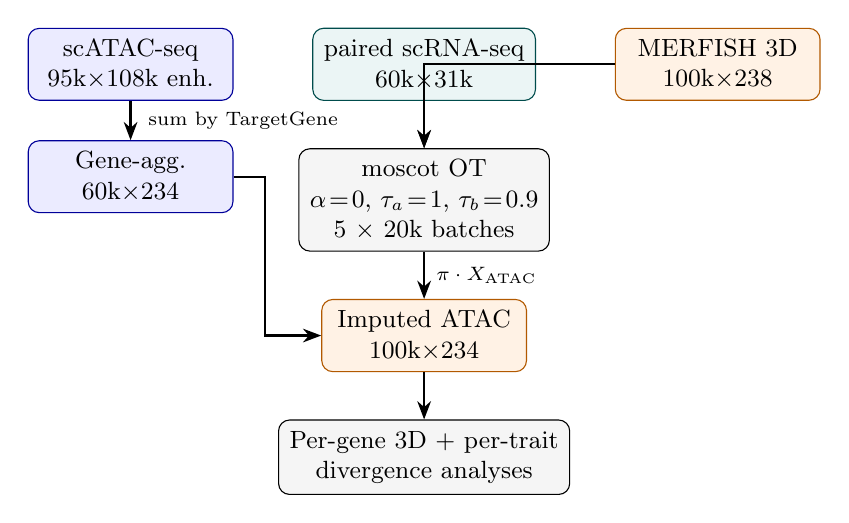
\begin{tikzpicture}[
  font=\small,
  every node/.style={align=center,rounded corners,inner sep=4pt},
  box/.style={draw,fill=gray!8,minimum width=2.6cm,minimum height=0.9cm},
  blue/.style={draw=blue!60!black,fill=blue!8,minimum width=2.6cm,minimum height=0.9cm},
  green/.style={draw=teal!60!black,fill=teal!8,minimum width=2.6cm,minimum height=0.9cm},
  orange/.style={draw=orange!70!black,fill=orange!10,minimum width=2.6cm,minimum height=0.9cm},
  arr/.style={-{Stealth},thick}
]
\node[blue]   (atac)   {scATAC-seq\\95k\(\times\)108k enh.};
\node[blue, below=0.5cm of atac] (atacg) {Gene-agg.\\60k\(\times\)234};
\node[green, right=1.0cm of atac] (rna)  {paired scRNA-seq\\60k\(\times\)31k};
\node[orange, right=1.0cm of rna] (mer)  {MERFISH 3D\\100k\(\times\)238};
\node[box, below=0.6cm of rna]   (ot)    {moscot OT\\\(\alpha\!=\!0\), \(\tau_a\!=\!1\), \(\tau_b\!=\!0.9\)\\5 \(\times\) 20k batches};
\node[orange, below=0.6cm of ot] (imp)   {Imputed ATAC\\100k\(\times\)234};
\node[box, below=0.6cm of imp]   (out)   {Per-gene 3D + per-trait\\divergence analyses};

\draw[arr] (atac) -- node[right,xshift=2pt]{\scriptsize sum by TargetGene} (atacg);
\draw[arr] (rna)  -- (ot);
\draw[arr] (mer)  -| (ot);
\draw[arr] (atacg.east) -- ++(0.4,0) |- (imp.west) node[pos=0.25,above,rotate=90]{};
\draw[arr] (ot)   -- node[right]{\scriptsize \(\pi\cdot X_\text{ATAC}\)} (imp);
\draw[arr] (imp)  -- (out);
\end{tikzpicture}
\caption{\textbf{Cross-modality optimal-transport pipeline.}
Paired scATAC-seq is gene-aggregated; the matched scRNA-seq is mapped onto the
3D MERFISH atlas via \emph{moscot} \citep{klein2025moscot}; the resulting
transport plan is reused on the ATAC matrix to produce per-gene chromatin
scores in 3D space.}
\label{fig:pipeline}
\end{figure}

\subsection{Per-gene and per-trait spatial concordance}

Aggregating the imputed per-gene ATAC scores by CHD trait
\citep{jin2017chd,homsy2015chd}, we obtain spatially smooth maps for all ten
traits passing the \(n_\text{genes}\!\ge\!3\) threshold
(Fig.~\ref{fig:traitsummary}). Cardiomyopathy traits show low signal in the
outflow/atrial region and elevated signal across the ventricular body, while
septal-defect and outflow-tract traits highlight the ventricular wall and
valvular regions, mirroring known disease anatomy.

\begin{figure}[t]
\centering
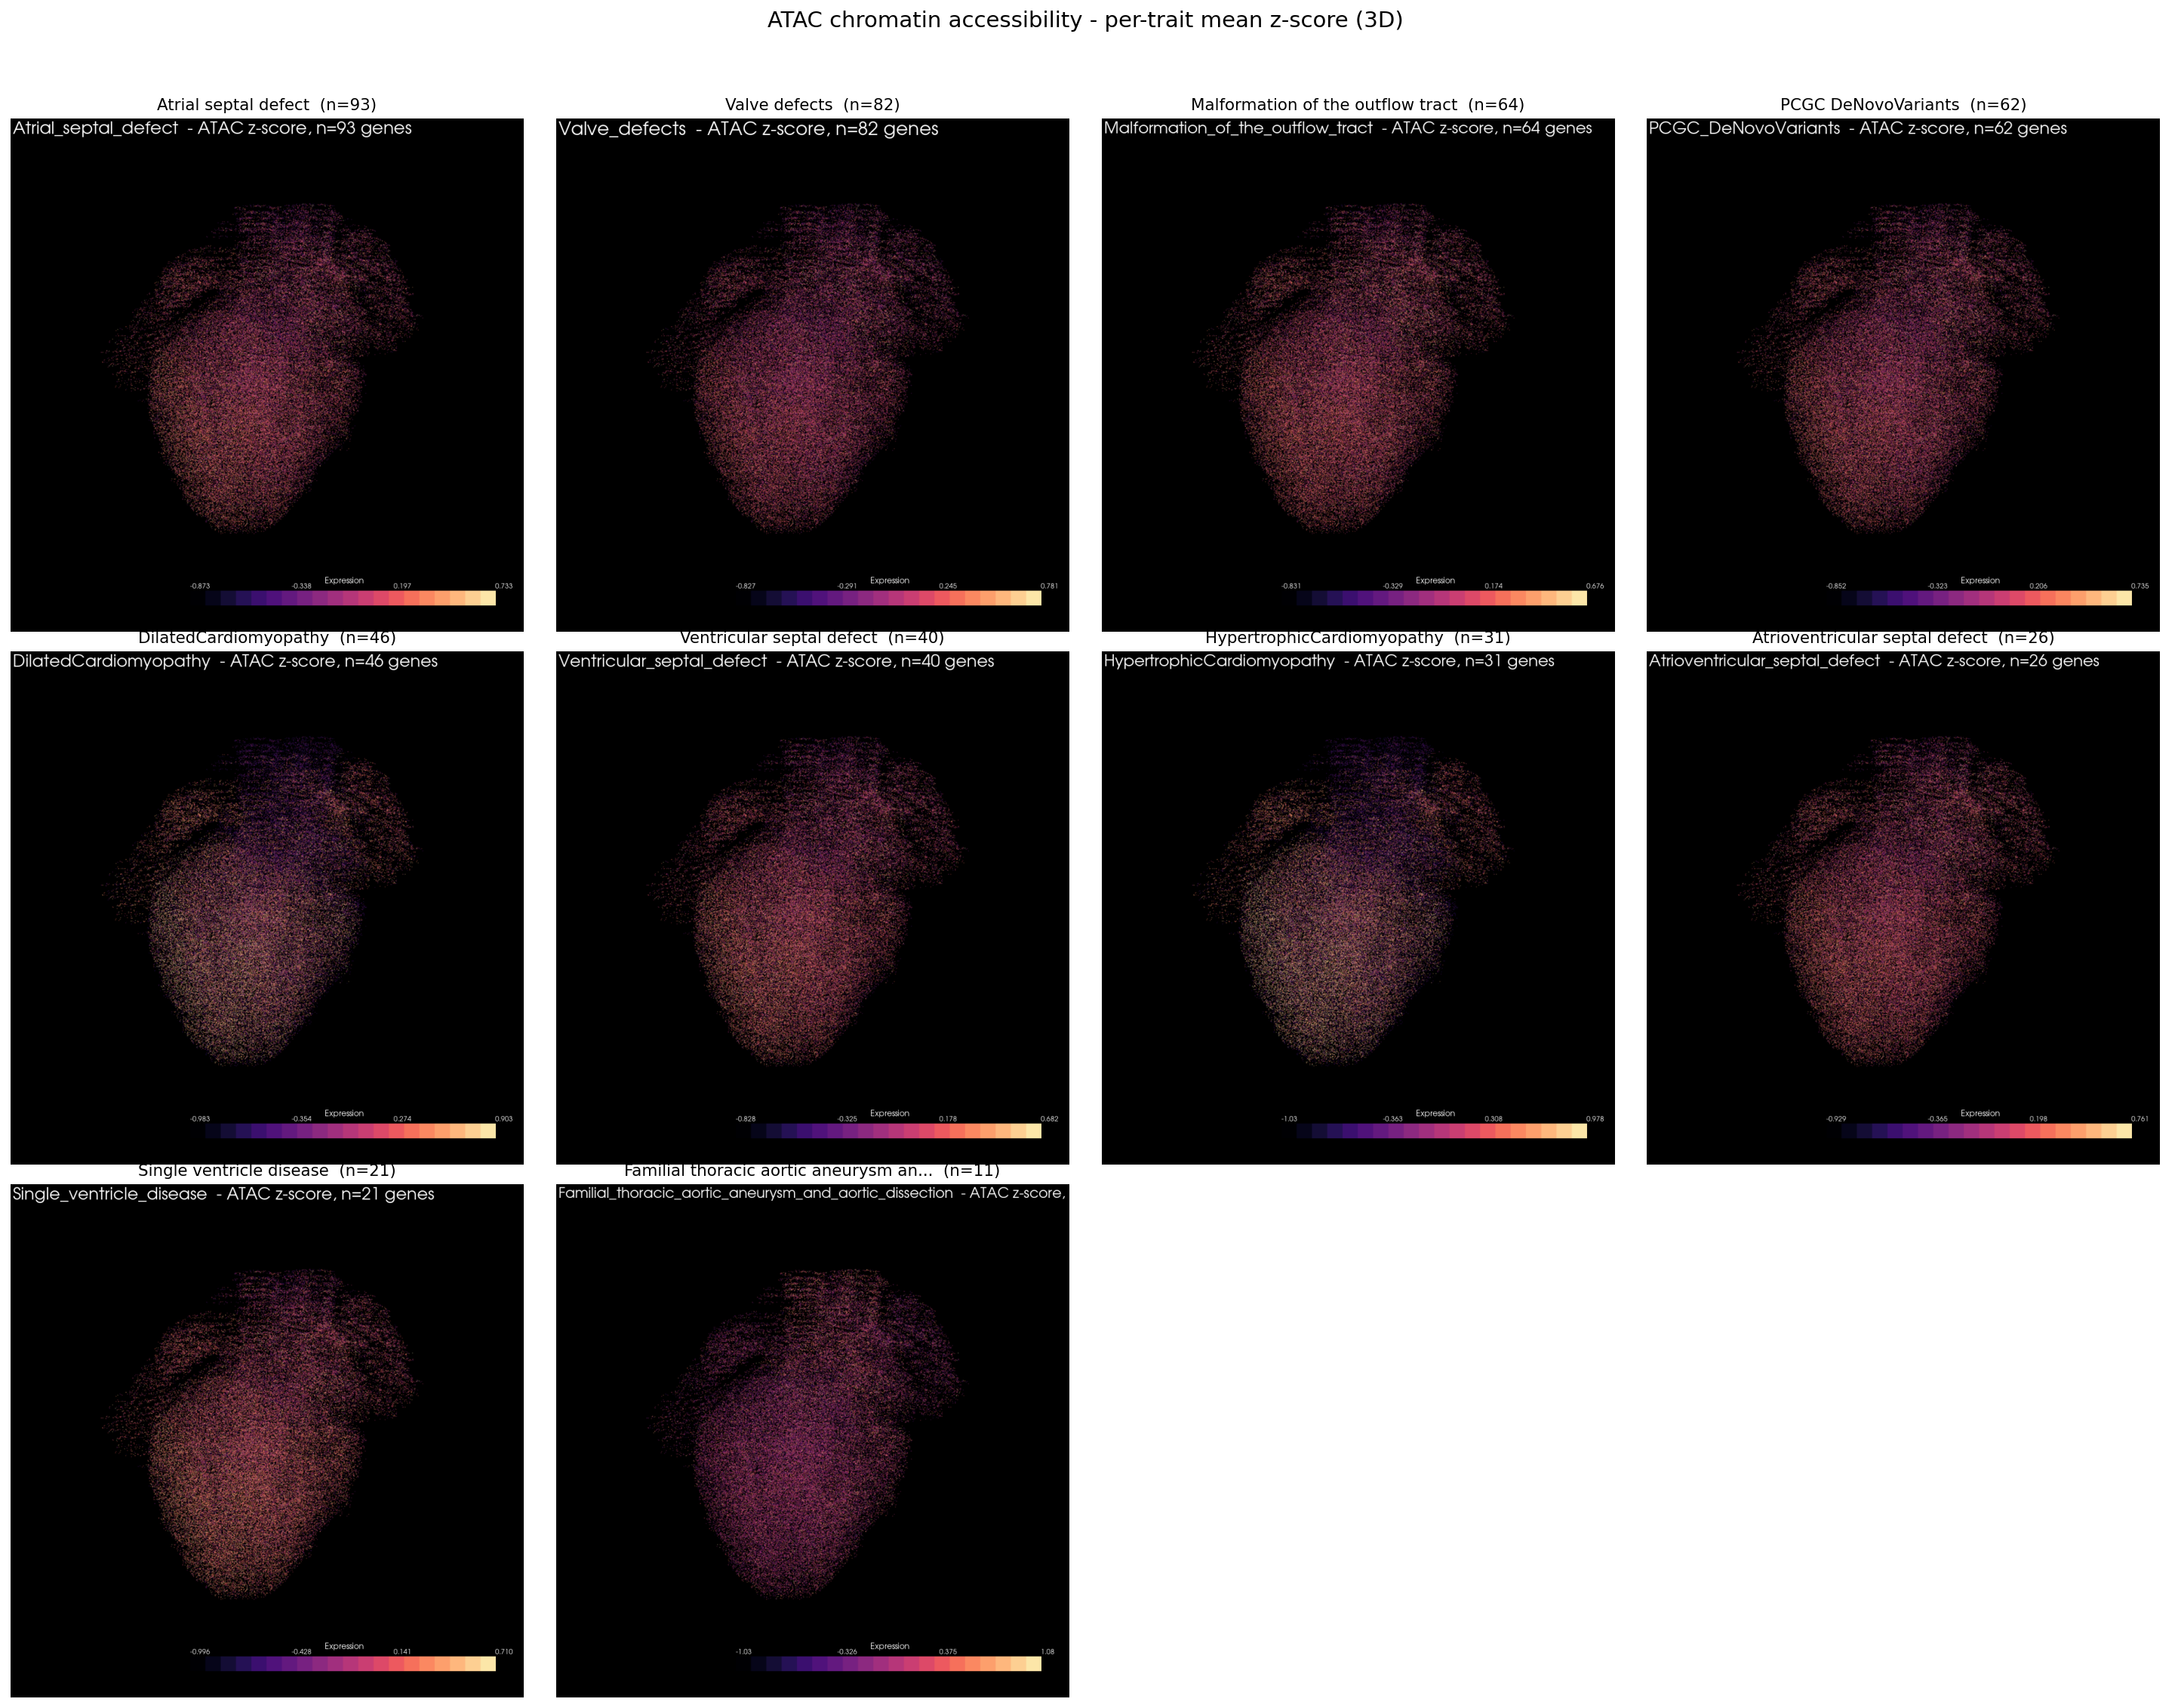
\includegraphics[width=\linewidth]{figures/fig2_trait_summary.png}
\caption{\textbf{3D ATAC trait maps (PCW 11--13).}
Per-cell mean \(z\)-score over genes assigned to each of the 10 CHD traits.
Apex points down. HCM and DCM concentrate in the ventricular body;
septal-defect and outflow traits highlight the wall/valve regions.}
\label{fig:traitsummary}
\end{figure}

To quantify how ATAC and RNA agree spatially, we computed the Pearson
correlation of imputed ATAC and imputed RNA across the 100{,}000 MERFISH cells
for each of 215 shared genes. The distribution is strongly right-skewed
(median \(r=0.13\); mean \(r=0.22\); Fig.~\ref{fig:gener}), with a clear
high-concordance tail dominated by sarcomere and cardiac-TF genes
(\emph{RBM20} \(r=0.87\); \emph{FHOD3} \(r=0.85\); \emph{LDB3} \(r=0.81\);
\emph{MYBPC3} \(r=0.81\) -- all classical hypertrophic / dilated cardiomyopathy
genes \citep{maron2018hcm}). Gene-level disagreement is concentrated in
broadly-expressed regulators (\emph{RPL5}, \emph{CHD4}, \emph{KDM5B}). At the
trait level (Table~\ref{tab:traitr}), HCM and DCM achieve the highest
concordance (\(r=0.79\), 0.73); septal and outflow traits, which span more
heterogeneous gene sets, give weaker but uniformly positive agreement
(\(r=0.34\)--0.42).

\begin{figure}[t]
\centering
\begin{subfigure}[t]{0.49\linewidth}
\centering
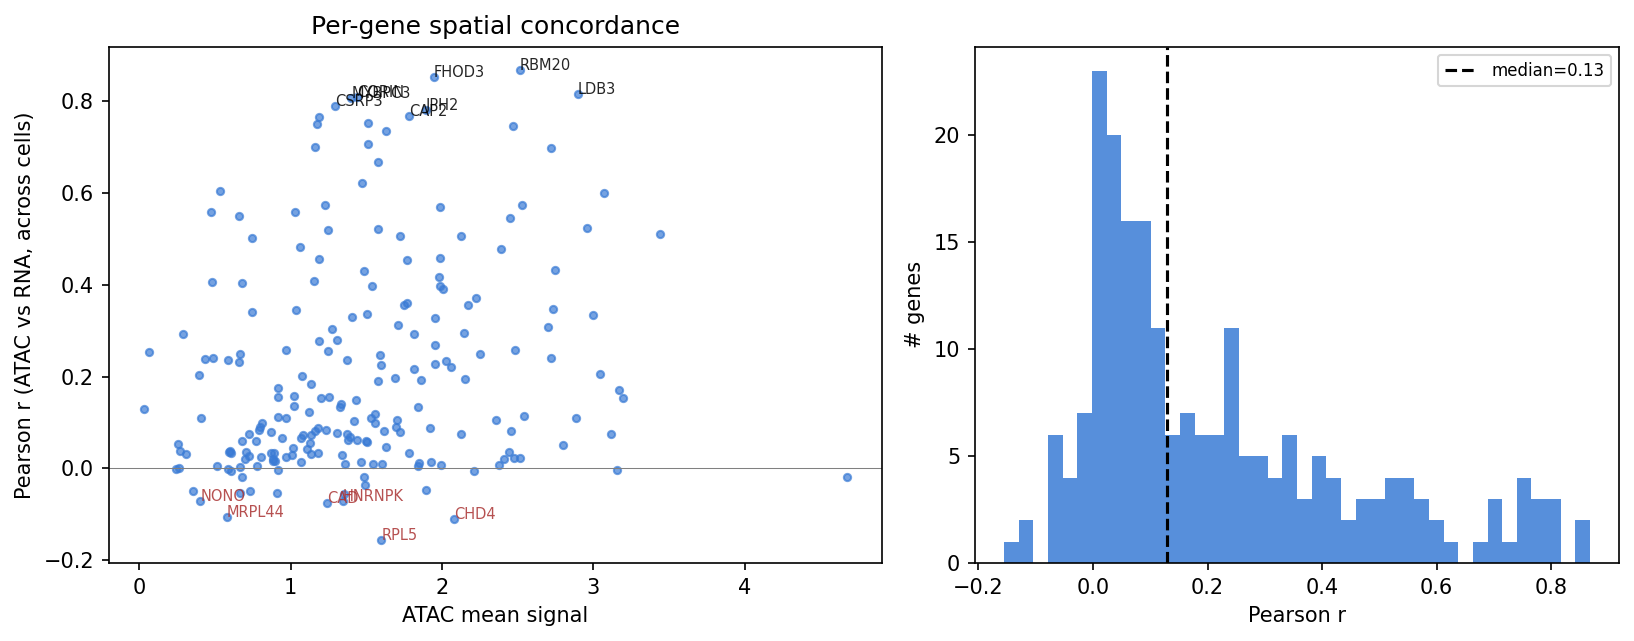
\includegraphics[width=\linewidth]{figures/fig3_gene_correlation.png}
\caption{Per-gene spatial \(r\), 215 shared genes.}
\label{fig:gener}
\end{subfigure}\hfill
\begin{subfigure}[t]{0.49\linewidth}
\centering
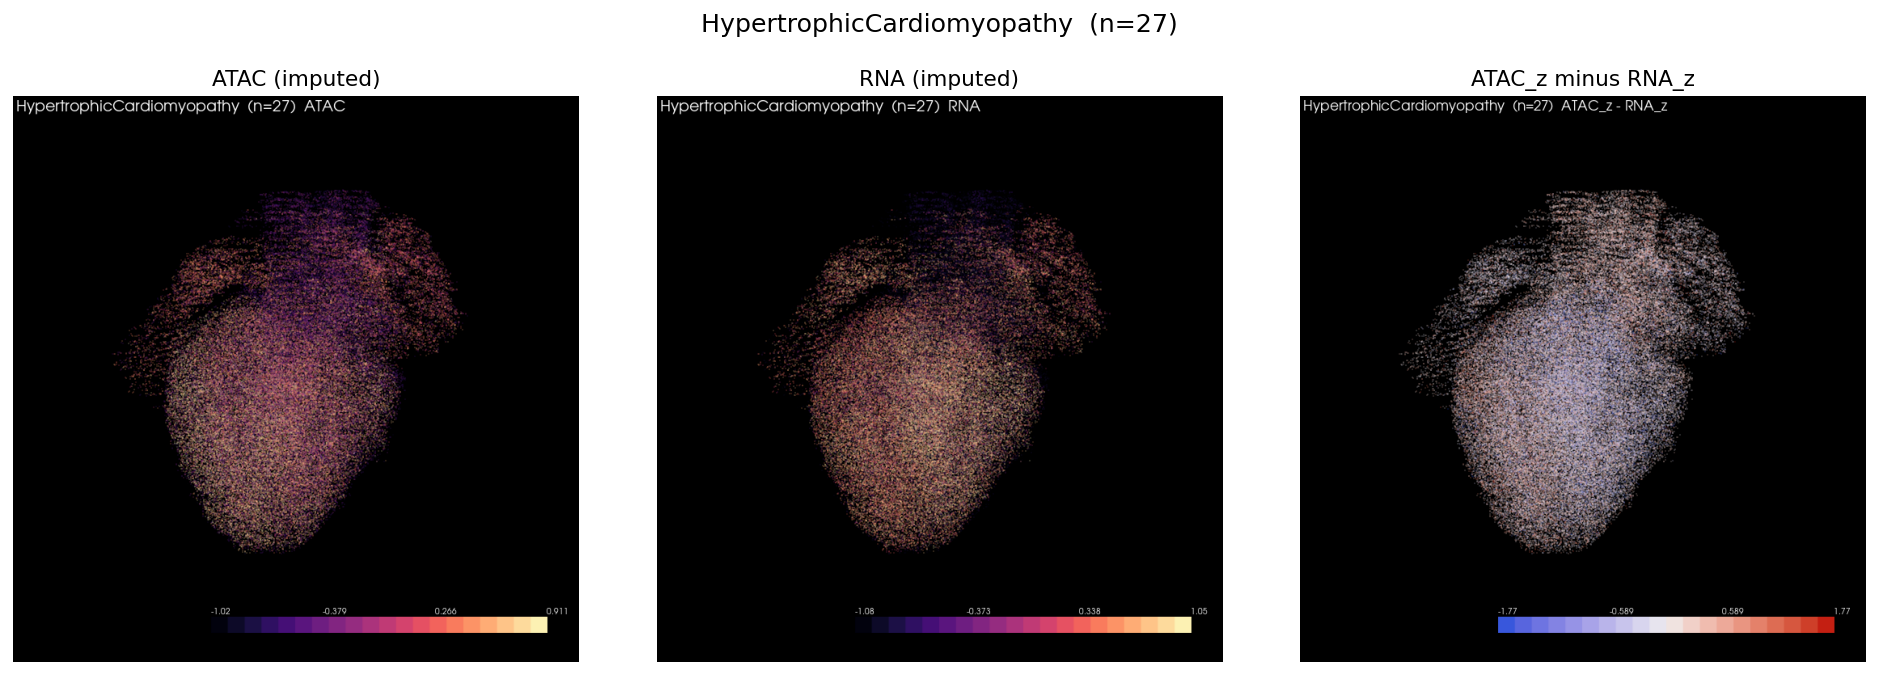
\includegraphics[width=\linewidth]{figures/fig4a_hcm_triptych.png}
\caption{HCM trait triptych: ATAC, RNA, ATAC\(_z\!-\!\)RNA\(_z\).}
\label{fig:hcm}
\end{subfigure}
\caption{\textbf{Per-gene and per-trait spatial concordance.}
(a) Histogram of per-gene Pearson \(r\) (median 0.13). Top genes are
sarcomeric / cardiomyopathy-associated. (b) For HCM, the three-panel
ATAC \(\vert\) RNA \(\vert\) divergence layout shows near-uniform
near-zero divergence -- the chromatin map and the RNA map carry the
same ventricular-CM gradient.}
\label{fig:concordance}
\end{figure}

\begin{table}[t]
\centering
\caption{\textbf{Per-trait spatial Pearson \(r\) (ATAC vs RNA).}
Cardiomyopathy traits dominated by sarcomeric genes show the strongest
concordance.}
\label{tab:traitr}
\small
\begin{tabular}{lrr}
\toprule
\textbf{Trait} & \textbf{n genes} & \textbf{Pearson \(r\)} \\
\midrule
Hypertrophic Cardiomyopathy           & 27 & \textbf{0.79} \\
Dilated Cardiomyopathy                & 40 & \textbf{0.73} \\
Familial Thoracic Aortic Aneurysm     & 9  & 0.42 \\
Valve defects                         & 74 & 0.40 \\
Outflow-tract malformation            & 57 & 0.38 \\
Atrial septal defect                  & 87 & 0.38 \\
Atrioventricular septal defect        & 22 & 0.36 \\
Single-ventricle disease              & 17 & 0.36 \\
PCGC de-novo variants                 & 57 & 0.36 \\
Ventricular septal defect             & 33 & 0.34 \\
\bottomrule
\end{tabular}
\end{table}

\subsection{Chromatin is broader than RNA: cell-type signal}

A 14\(\times\)22 dot plot of the highlight gene panel by coarse cell type
(Fig.~\ref{fig:dotplot}) shows the canonical chromatin priming signature
\citep{wamstad2012priming,paige2012priming}: classical sarcomere genes
(\emph{MYBPC3}, \emph{MYL2}, \emph{TNNT2}, \emph{TNNI3}, \emph{TNNC1},
\emph{ACTC1}, \emph{ACTN2}, \emph{TPM1}) are RNA-restricted to ventricular and
atrial cardiomyocytes, but their CHD-enhancer ATAC signal is detectable across
multiple lineages including epicardial, endocardial and mural cells. RNA is
sharp and lineage-restricted; chromatin is graded and permissive.

\begin{figure}[t]
\centering
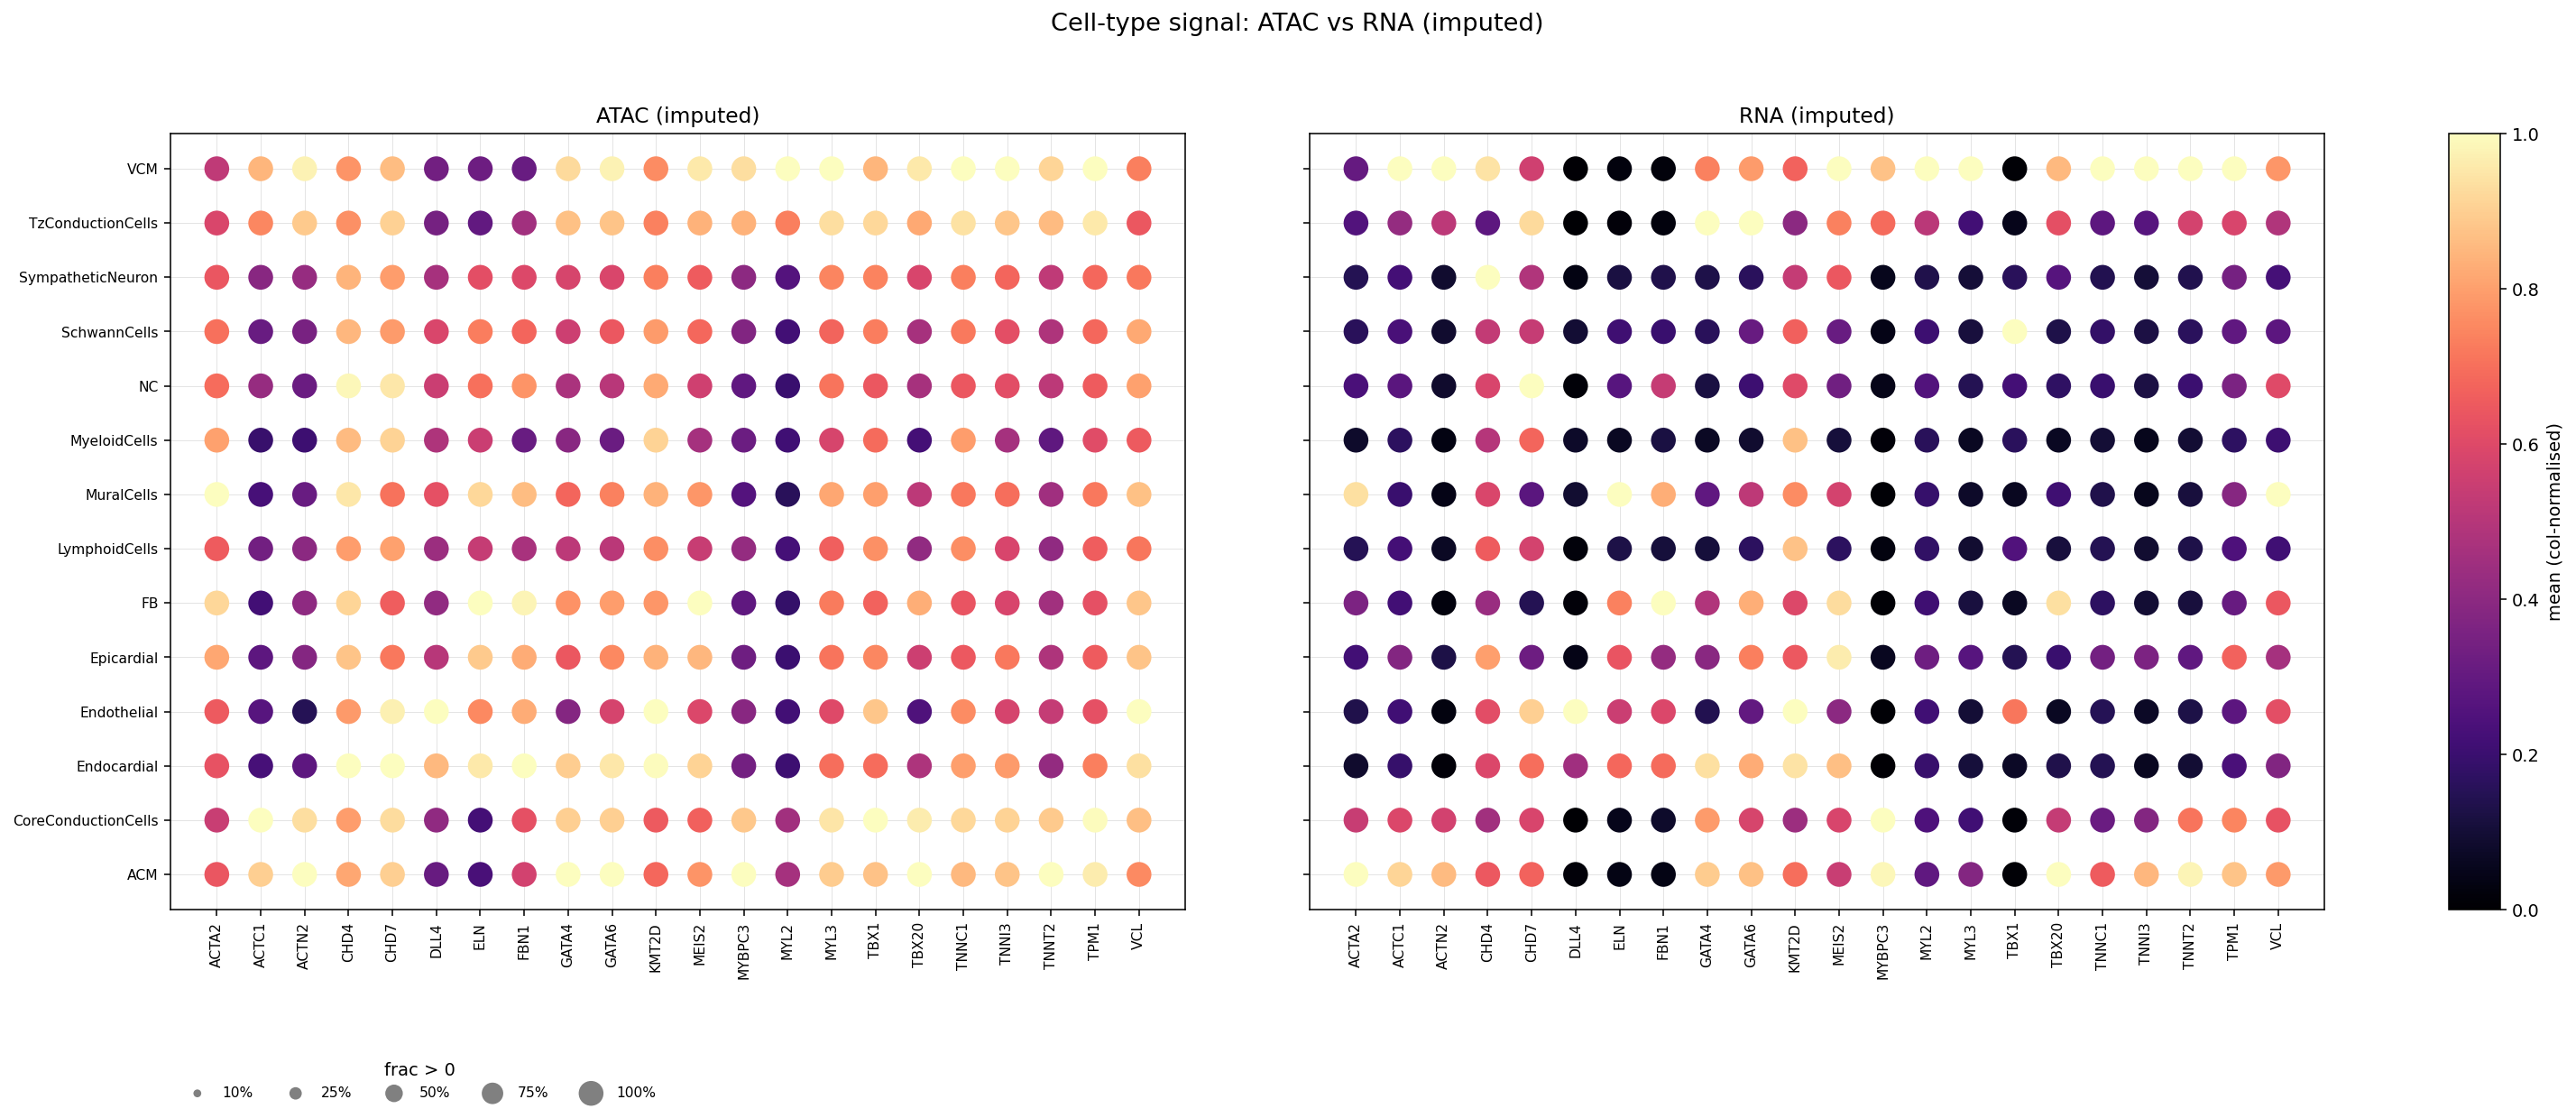
\includegraphics[width=\linewidth]{figures/fig5_celltype_dotplot.png}
\caption{\textbf{Cell-type dot plot, ATAC vs RNA.}
Two panels (ATAC, left; RNA, right), 14 coarse cell types \(\times\) 22
highlight genes. Color: column-normalised mean signal; size: fraction
expressing. Sarcomeric genes are strongly RNA-specific to VCM/ACM but are
chromatin-accessible across multiple cardiac lineages.}
\label{fig:dotplot}
\end{figure}

\subsection{Within-lineage decoupling of ATAC and RNA}

The cell-type-resolved view raises a sharper question: is the global per-gene
\(r=0.13\) driven by between-lineage means (which the dot plot shows are
correlated) or by within-lineage spatial co-variation? Restricting Pearson
\(r\) to cells \emph{inside each coarse lineage} answers this directly
(Fig.~\ref{fig:withinct}). Median within-lineage \(r\) ranges from 0.034
(SchwannCells) to 0.076 (ACM); all 14 lineages have median \(r<0.08\). Even
genes with high global \(r\) collapse: \emph{MYL2} drops from \(r=0.77\)
globally to \(r=0.24\) within VCMs, and \emph{GATA4} from \(r=0.51\) to
\(r\!\approx\!0\) (Fig.~\ref{fig:gata4}). Within VCMs, GATA4 chromatin is
uniformly accessible (orange across the lineage) while RNA is uniformly low
and varies independently of chromatin -- a textbook decoupling pattern.

\begin{figure}[t]
\centering
\begin{subfigure}[t]{0.55\linewidth}
\centering
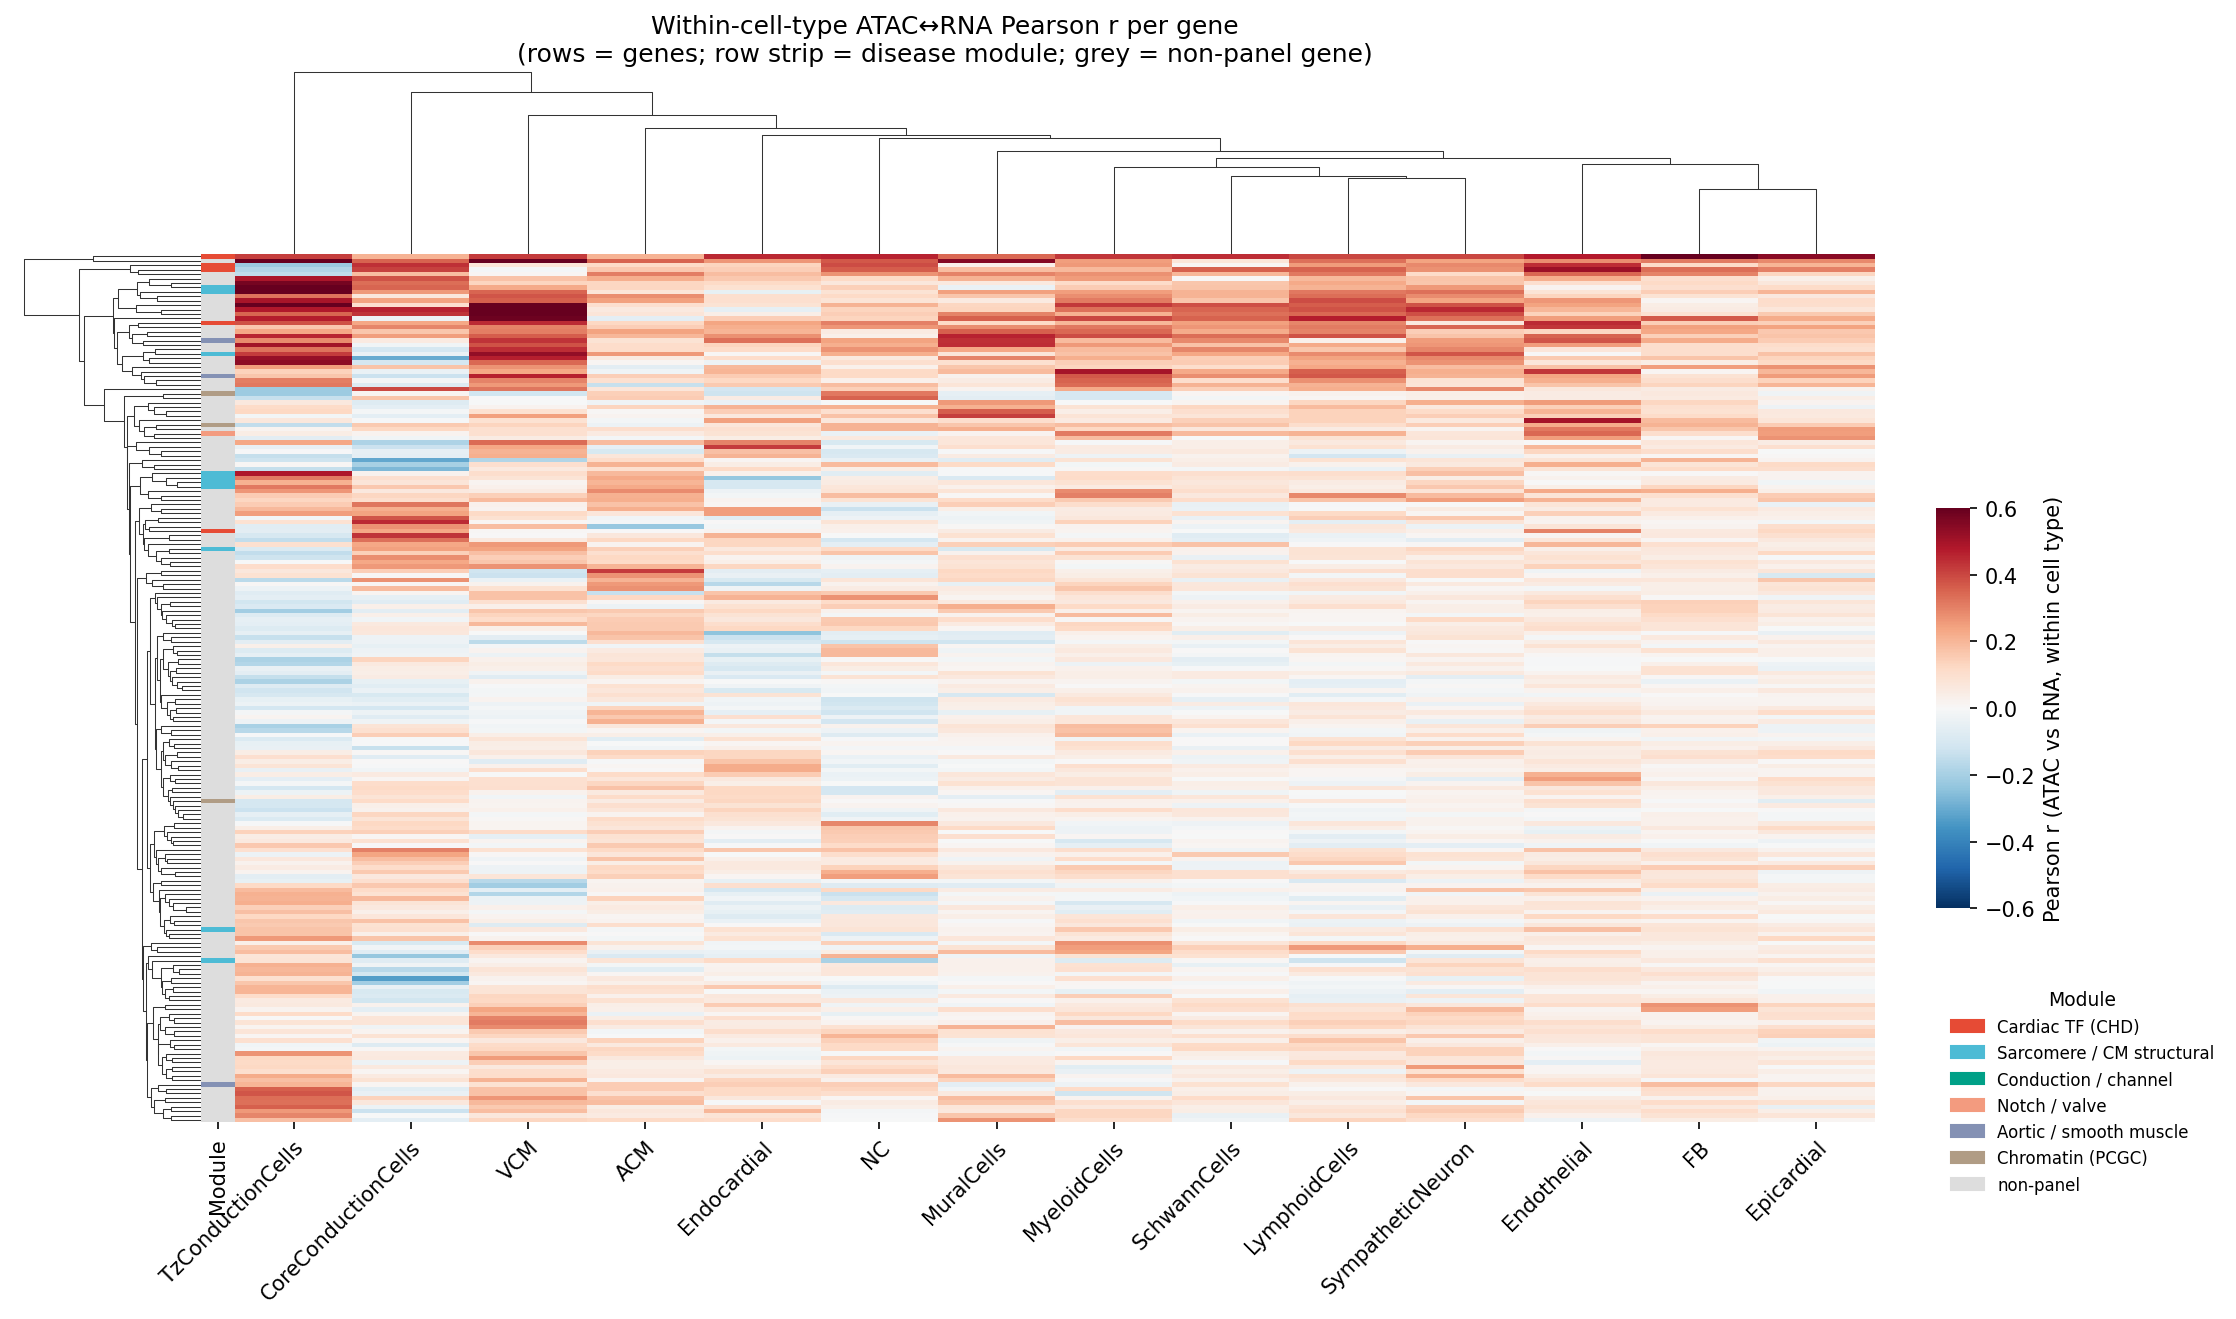
\includegraphics[width=\linewidth]{figures/fig6_within_ct_pearson.png}
\caption{Within-lineage Pearson \(r\), 215 \(\times\) 14 clustermap.}
\label{fig:withinct}
\end{subfigure}\hfill
\begin{subfigure}[t]{0.42\linewidth}
\centering
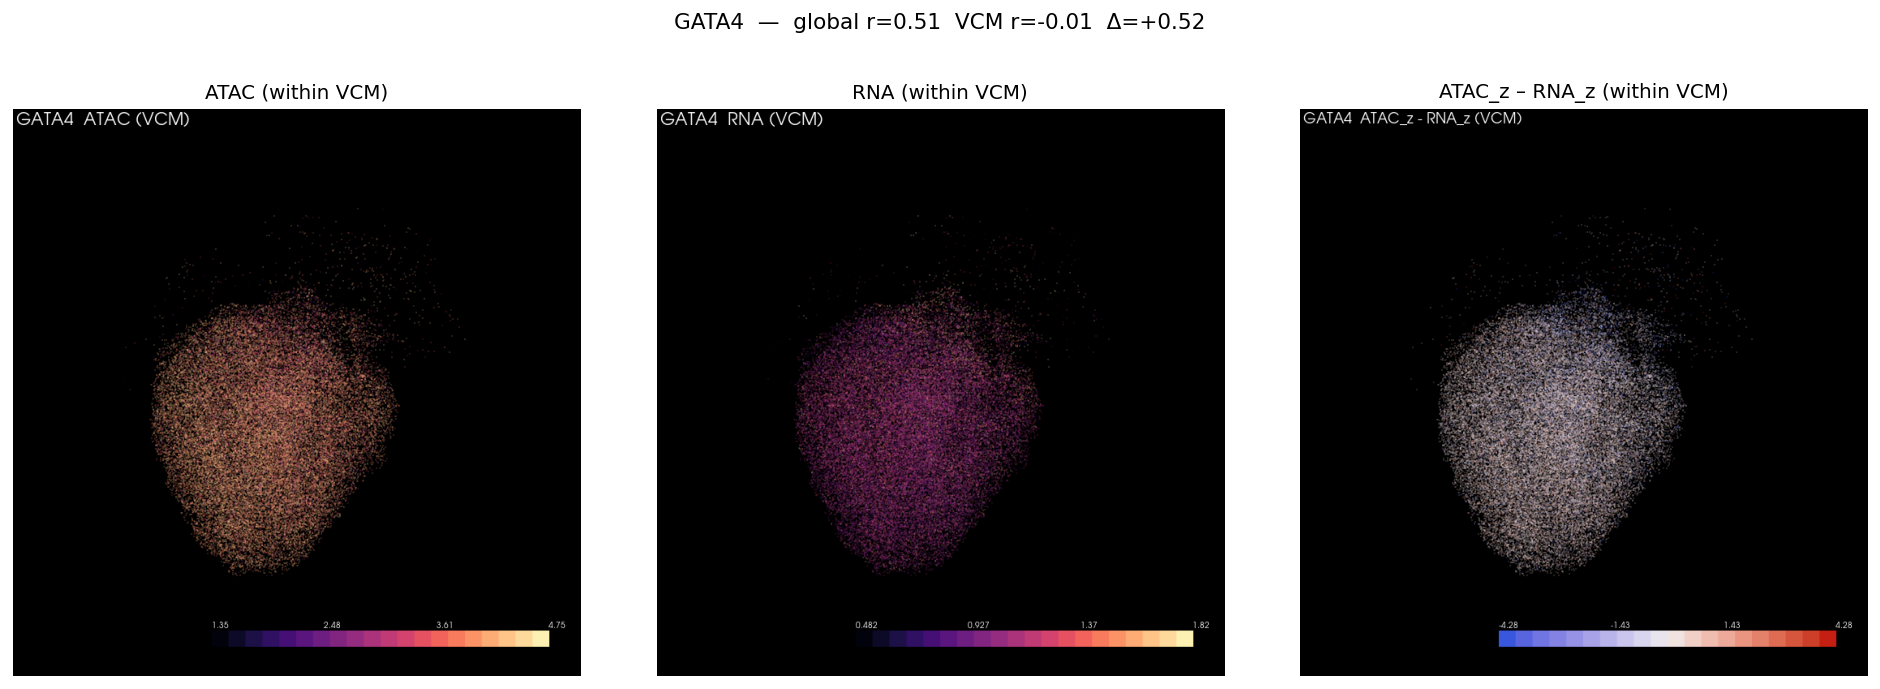
\includegraphics[width=\linewidth]{figures/fig9_gata4_within_vcm.png}
\caption{\emph{GATA4} within VCMs.}
\label{fig:gata4}
\end{subfigure}
\caption{\textbf{Within-lineage chromatin--RNA decoupling.}
(a) Per-gene Pearson \(r\) recomputed inside each coarse lineage. All 14
column-medians lie between 0.03 and 0.08; the global \(r=0.13\) signal is
dominated by between-lineage means. (b) For \emph{GATA4} restricted to
VCMs (\(n=48{,}595\)), chromatin is uniformly open (left panel) while RNA
is uniformly low (centre); the divergence map (right) shows their spatial
patterns are independent.}
\label{fig:within}
\end{figure}

\subsection{ATAC is spatially broader than RNA for sarcomere genes}

To formalise the qualitative dot-plot observation, we computed the spatial
spread (radius of gyration of top-decile cells) per gene per modality
(Fig.~\ref{fig:spread}). Of 213 non-trivial genes, 115 have ATAC spread
\(>\) RNA spread (median \(\Delta r_g = +10.8\), median centroid shift
\(=358\) units). The Sarcomere/CM-structural cluster (\emph{MYL2}, \emph{MYL3},
\emph{ACTN2}, \emph{ACTC1}, \emph{TPM1}, \emph{TNNC1}, \emph{TNNI3}) sits as a
coherent group above the diagonal, the strongest deviation in the panel. This
constitutes direct evidence of priming: chromatin at structural CM genes is
permissive in lineages where these transcripts are not yet expressed.

\begin{figure}[t]
\centering
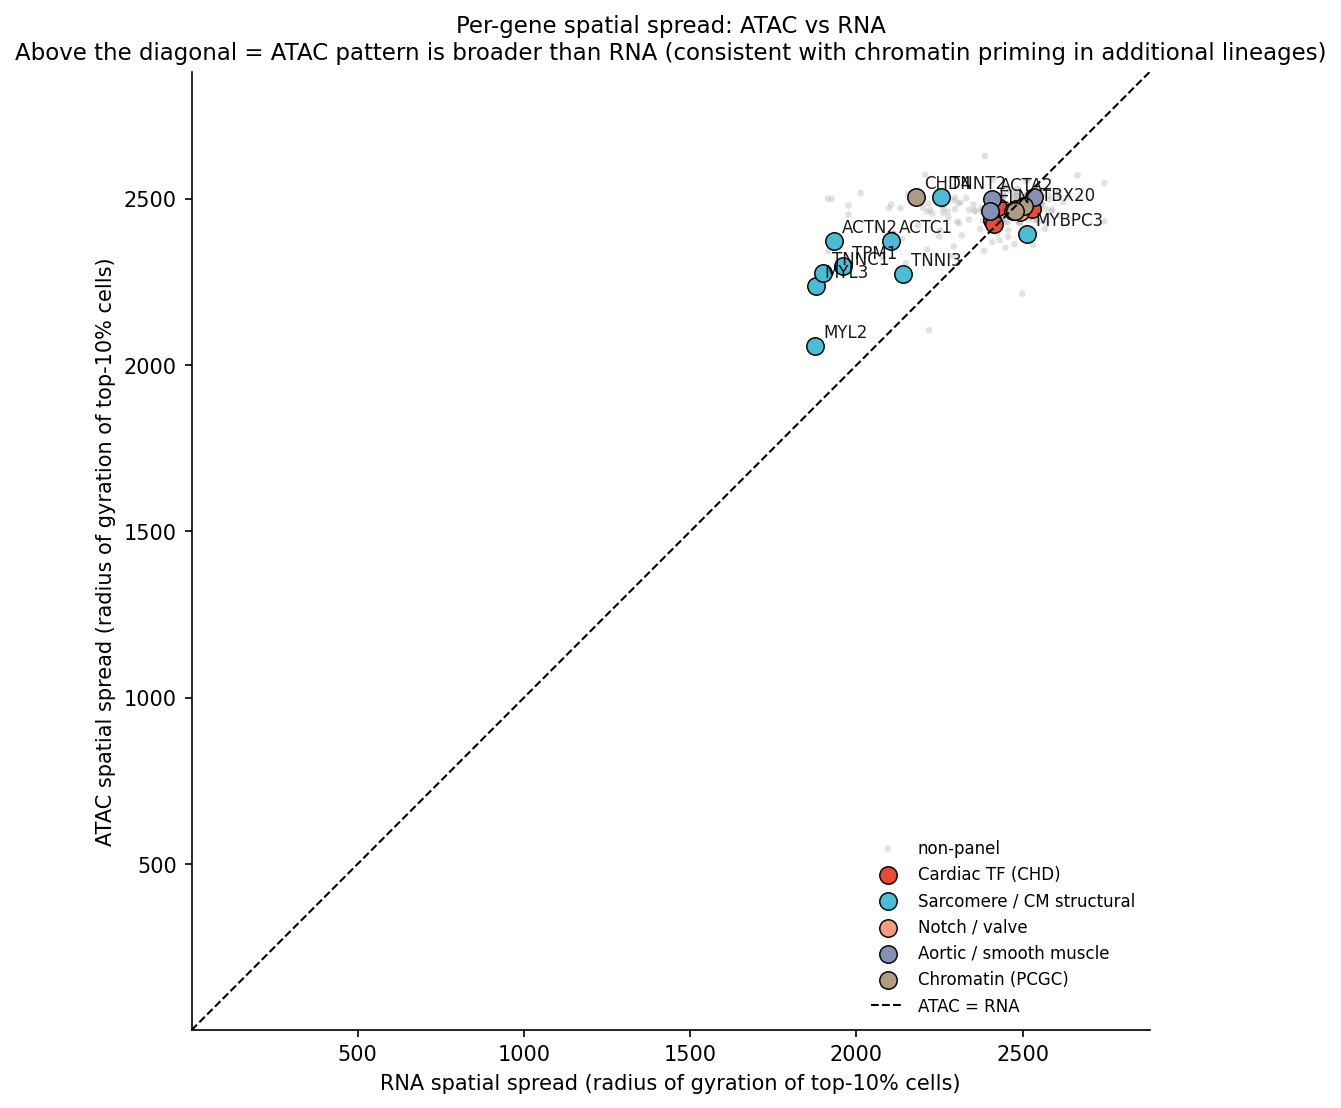
\includegraphics[width=0.78\linewidth]{figures/fig7_spatial_spread.png}
\caption{\textbf{Spatial spread of ATAC vs RNA, per gene.}
\(x\)-axis: radius of gyration of the top-decile RNA cells; \(y\)-axis: same
for ATAC. Dashed = identity. Sarcomere genes (cyan: MYL2, MYL3, ACTN2,
ACTC1, TPM1, TNNC1, TNNI3) are systematically above the diagonal --
chromatin spans a larger anatomical territory than transcription.}
\label{fig:spread}
\end{figure}

\subsection{Priming asymmetry separates two gene classes}

A per-cell quadrant classification (\(\mathrm{ATAC}_z>+1\) vs
\(\mathrm{RNA}_z<0\) and vice versa) yields per-gene fractions of
``primed-only'' and ``expressed-without-priming'' cells. Ranking genes by
each fraction (Fig.~\ref{fig:priming}) splits the panel cleanly: the top
primed-only genes are early developmental TFs and signalling regulators
(\emph{TBX1}, \emph{NODAL}, \emph{SALL4}, \emph{STRA6}, \emph{CHD4},
\emph{FLT4}) -- exactly the gene class with established
poised-chromatin behaviour during cardiogenesis
\citep{wamstad2012priming,paige2012priming}. The top expressed-only genes
are housekeeping or chromatin-modifier regulators (\emph{RPL5}, \emph{ZEB2},
\emph{NONO}, \emph{RAD21}, \emph{HNRNPK}, \emph{KDM6A}, \emph{KDM5B}), whose
broad RNA expression is driven by promoter-proximal regulation that the
CHD-\emph{enhancer} panel does not interrogate. The conduction-system
cardiomyocyte rows (CoreConductionCells, TzConductionCells) are the brightest
in the primed-only column for sarcomere genes (\emph{ACTC1}, \emph{TNNC1},
\emph{TNNI3}, \emph{MYL3}), consistent with these specialised non-contractile
cardiomyocytes maintaining accessible structural-gene chromatin while
suppressing transcription \citep{christoffels2009conduction}.

\begin{figure}[t]
\centering
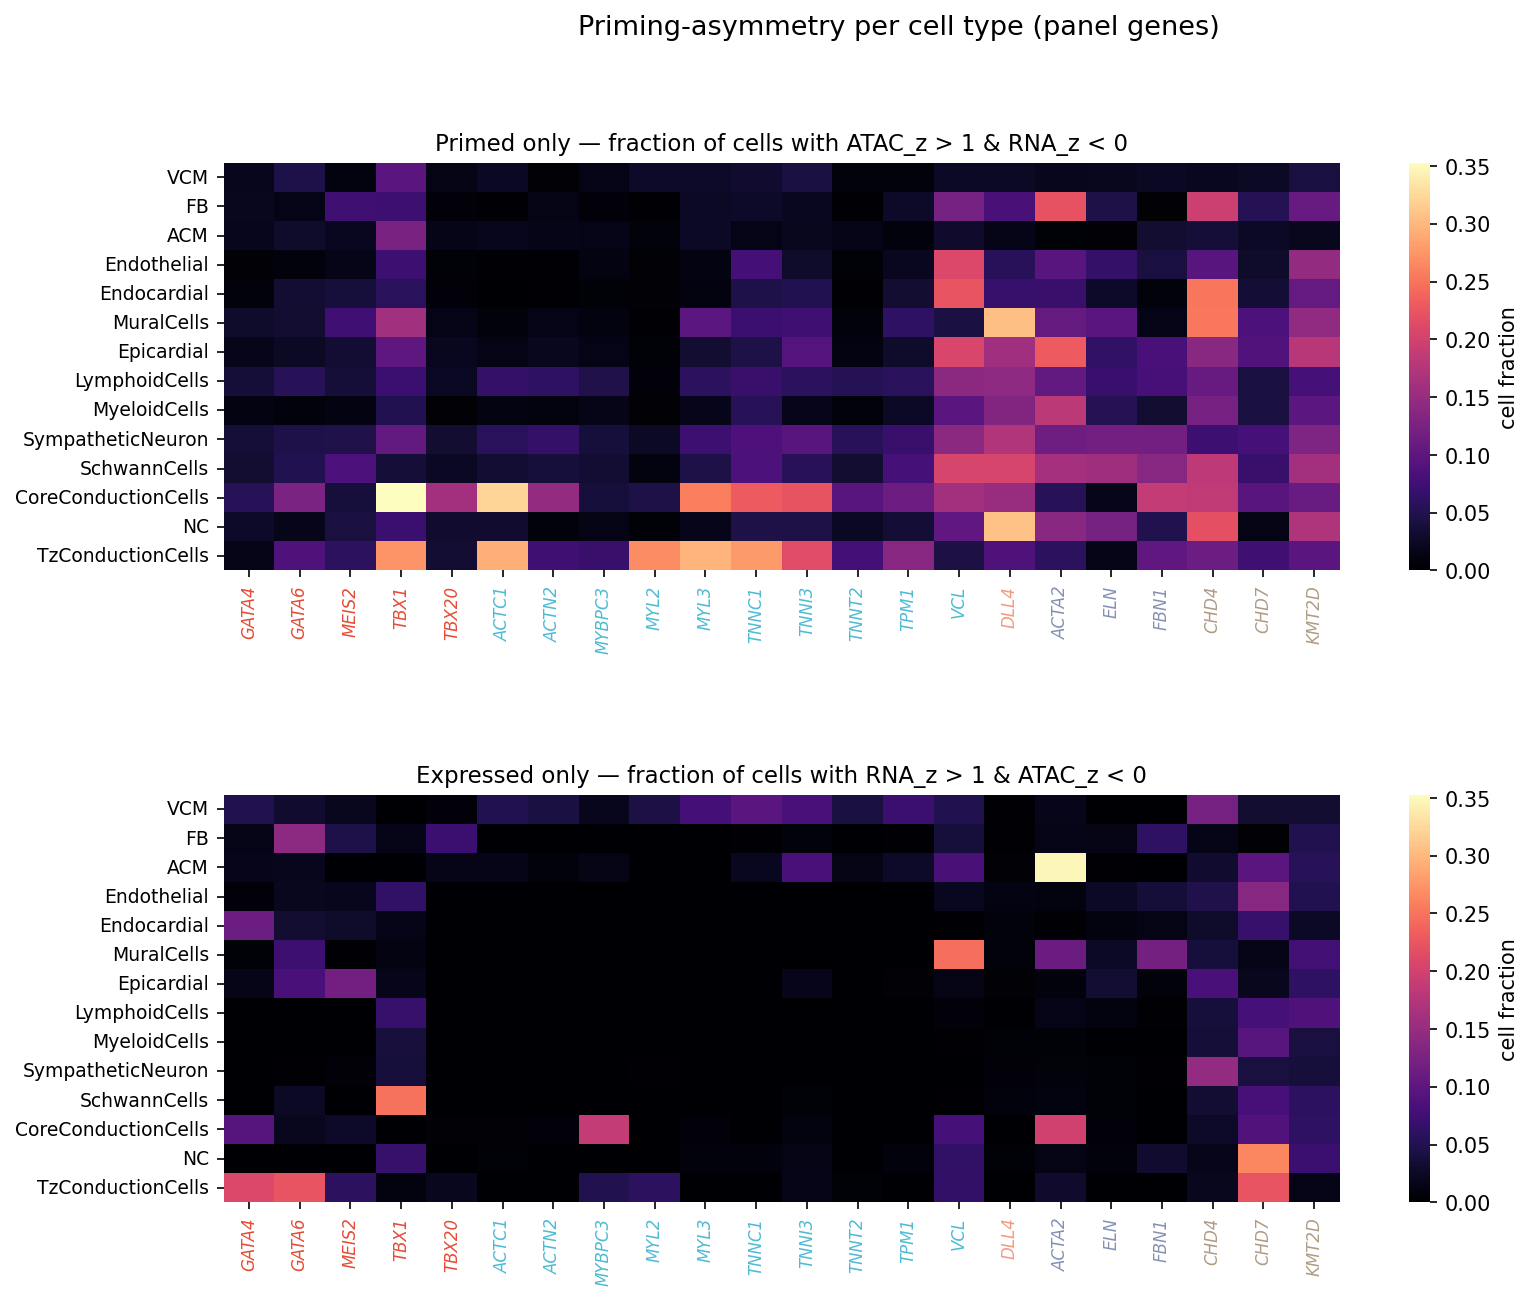
\includegraphics[width=\linewidth]{figures/fig8_priming_quadrant.png}
\caption{\textbf{Cell-type priming-asymmetry heatmap.}
14 coarse lineages \(\times\) the 22-gene highlight panel, two stacks:
fraction of primed-only cells (left) and expressed-without-priming cells
(right). Conduction-system cardiomyocytes show the highest primed-only
fractions for sarcomere genes; ACMs and VCMs dominate the expressed-only
panel for the same genes.}
\label{fig:priming}
\end{figure}

% =====================================================================
\section{Discussion}

We present, to our knowledge, the first 3D spatial map of CHD-enhancer
chromatin accessibility in the developing human heart. The cross-modality
re-use of an optimal-transport plan -- solving on RNA, applying to ATAC --
sidesteps the absence of true paired ATAC--MERFISH data and gives a per-gene
chromatin score on the same anatomical grid as the RNA atlas. The pipeline
runs in minutes on a single CPU and is conceptually portable to any paired
multimodal scenario where one modality already has a transport plan to a
spatial reference.

The biology that emerges is internally consistent across four orthogonal
analyses. Cardiomyopathy traits show high ATAC--RNA concordance because the
sarcomere programme is sharply lineage-restricted in both modalities. CHD
traits with broader gene sets (septal, outflow, valve) show partial
concordance because their gene sets mix lineage-restricted (\emph{TBX5},
\emph{GATA4}, \emph{NKX2-5}) and broadly active regulators. Once we condition
on lineage, chromatin and RNA decouple almost completely: the within-lineage
\(r\) is essentially zero for all 14 coarse cell types. ATAC spreads further
in space than RNA for the very sarcomere genes that are most lineage-specific
in transcription. And the priming asymmetry separates two gene classes whose
behaviours have independent literature support
\citep{wamstad2012priming,paige2012priming,ameen2022cardiogenesis}:
developmental TFs are pre-marked at the chromatin level in lineages that do
not yet transcribe them, while housekeeping regulators show the inverse, in
agreement with promoter-proximal -- rather than distal-enhancer -- control.

The conduction-system finding deserves emphasis. Core and transitional
conduction cardiomyocytes carry chromatin accessible at structural sarcomere
loci that they actively repress at the RNA level. This is the molecular
counterpart to a long-standing developmental observation: conduction-system
cardiomyocytes derive from a working-myocardium-like precursor and
subsequently silence the contractile programme to acquire their electrical
identity \citep{christoffels2009conduction}. The chromatin map suggests that
silencing leaves the underlying enhancer landscape largely intact -- a
priming reservoir that may remain functionally relevant in
adult conduction-system pathology.

Three caveats apply. (i) The CHD-\emph{enhancer} input panel by construction
under-represents promoter-proximal regulation; ``expressed-without-priming''
genes should not be over-interpreted as truly unprimed. (ii) MOSCOT mapping
confidence (median 0.44) is high enough to recover bulk cell-type structure
but is not equivalent to true paired ATAC-MERFISH measurement; per-cell
chromatin scores are smoothed by the transport plan. (iii) Our analysis
covers PCW 11--13. Whether the same priming pattern holds at earlier
specification stages or persists into the late-fetal / post-natal heart
\citep{litvinukova2020adultheart} requires longitudinal data not yet
publicly available.

Notwithstanding, this work demonstrates that a CHD-enhancer chromatin
landscape can be resolved at single-cell, single-gene, three-dimensional
resolution by re-using an OT plan; that the resulting map is biologically
coherent at the trait, lineage, gene and anatomical level; and that the
\emph{difference} between chromatin and RNA -- not just their agreement -- is
where the developmental biology of CHD enhancers is most clearly visible.

% =====================================================================
\section{Methods}

\subsection{Data sources}
\begin{itemize}[leftmargin=1.2em,topsep=0pt,itemsep=2pt]
\item \texttt{chd\_enhancers\_counts.h5ad}: 95{,}684 cells \(\times\) 108{,}681
      enhancer features (paired multiome ATAC).
\item \texttt{all\_healthy\_PCW11-13.h5ad}: 95{,}684 cells \(\times\) 31{,}019
      genes (paired multiome RNA, raw counts).
\item \texttt{chd\_enhancer\_gene\_map.tsv}: enhancer \(\rightarrow\)
      \emph{TargetGene} mapping (108{,}681 \(\rightarrow\) 234 unique genes).
\item \texttt{heart\_disease\_genes.tsv}: gene \(\rightarrow\) trait labels for
      ten CHD-related traits.
\item MERFISH atlas: 100{,}000 cells \(\times\) 238 genes,
      \texttt{obsm["X\_spateo\_update"]} 3D coordinates, coarse cell-type and
      mapped fine cell-type labels (\(n=14\) and \(n=99\), respectively).
\end{itemize}

\subsection{Paired RNA/ATAC preparation
(\texttt{13\_prepare\_atac\_rna\_paired.py})}
Enhancer counts are aggregated to gene-level via a sparse boolean aggregator
\(A\) so that \(\mathrm{ATAC}_\mathrm{gene}=\mathrm{ATAC}_\mathrm{enh}\!\cdot\!A\).
Library-size normalisation
(\texttt{normalize\_total(target\_sum=1e4)}) and \texttt{log1p} are applied.
Cells with \(10\le n_\text{genes\_by\_counts}\le 200\) are kept (60{,}187 of
95{,}684; 62.9\%). RNA and ATAC share \texttt{obs\_names} exactly and are
realigned to the post-QC ATAC ordering.

\subsection{MOSCOT cross-modality imputation
(\texttt{14\_moscot\_atac\_imputation.py})}
We use \emph{moscot} \citep{klein2025moscot}, building on optimal-transport
formulations from \citet{schiebinger2019waddingtonot} and
\citet{demetci2022scot}. The OT source is the paired RNA matrix (60{,}187
cells, log-normalised) on the 229 features shared with MERFISH (after dropping
8 S/G2M cell-cycle genes). MERFISH is split into 5 batches of 20{,}000 cells.
For each batch we instantiate a \texttt{MappingProblem} with
\texttt{xy\_callback="local-pca"} and solve with \(\alpha=0\) (purely
quadratic), \(\tau_a=1\) (balanced source), \(\tau_b=0.9\) (semi-relaxed
target), on JAX-CPU. The transport matrix is rescaled by the spatial batch
size, \(\pi \leftarrow \pi \cdot n_{\text{sp,batch}}\), then the imputed ATAC
for the batch is \(\pi\!\cdot\!X_\text{ATAC}\). Cell-type labels are
transferred via \(\pi\!\cdot\!\mathrm{onehot}(\text{celltype})\). Per-batch
solve takes \(\sim\!110\) s; total runtime \(\sim\!10\) min.

\subsection{3D visualisation and trait aggregation
(\texttt{15\_atac\_3d\_visualization.py})}
Each of the 234 imputed ATAC genes is rendered as a 3D scatter (z-axis flipped
so apex points down) using \emph{Scanpy}/\emph{matplotlib}
\citep{wolf2018scanpy,virshup2023scverse}. Per-trait scores are computed by
\(z\)-scoring each contributing gene across cells and averaging within each
trait gene set (\(n_\text{genes}\!\ge\!3\) required; all 10 traits qualify).

\subsection{Divergence analyses
(\texttt{21\_atac\_rna\_3d\_divergence\_explore.py})}
Four analyses on the 215 genes shared between
\texttt{adata\_imputed\_atac.h5ad} and
\texttt{adata\_imputed\_disease\_genes.h5ad}, both on the 100{,}000-cell
MERFISH grid:
\begin{itemize}[leftmargin=1.2em,topsep=0pt,itemsep=2pt]
\item \textbf{(A) Spatial divergence atlas.} Per-cell panel-mean
      \(\lvert\mathrm{ATAC}_z-\mathrm{RNA}_z\rvert\) over the 22-gene CHD
      panel; module-level signed maps for six modules.
\item \textbf{(B) Priming-asymmetry quadrant analysis.} Per (gene, cell)
      classification: Primed (\(\mathrm{ATAC}_z>+1\) and \(\mathrm{RNA}_z<0\)),
      Expressed (\(\mathrm{RNA}_z>+1\) and \(\mathrm{ATAC}_z<0\)), Both, or
      Neither; per-gene rankings and per-cell-type heatmap.
\item \textbf{(C) Within-lineage Pearson \(r\).} For each of 14 coarse cell
      types, recompute per-gene Pearson \(r\) restricted to that lineage,
      yielding a 215\(\times\)14 matrix; four within-VCM divergent triptychs
      (\emph{DSP}, \emph{ACTC1}, \emph{MYL2}, \emph{GATA4}).
\item \textbf{(D) Spatial spread.} Per gene per modality, take the top-decile
      cells, compute the centroid and the radius of gyration over the 3D
      coordinates; scatter ATAC \(r_g\) vs RNA \(r_g\).
\end{itemize}
All quantities are computed without further smoothing of the imputed
matrices.

\subsection{Software and code availability}
Implementation: Python 3.11; \emph{moscot} \citep{klein2025moscot};
\emph{Scanpy} \citep{wolf2018scanpy}; \emph{anndata} / \emph{scverse}
\citep{virshup2023scverse}; JAX-CPU. Scripts (numbered 13--21) are in
\texttt{PCW12\_analysis/scripts/} of the project repository. Per-figure
provenance and TSV summaries accompany each output directory under
\texttt{PCW12\_analysis/figures/}.

% =====================================================================
\bibliographystyle{plainnat}
\bibliography{refs}

\end{document}
